\documentclass[conference]{IEEEtran}
\IEEEoverridecommandlockouts
% The preceding line is only needed to identify funding in the first footnote. If that is unneeded, please comment it out.
\usepackage{cite}
\usepackage{amsmath,amssymb,amsfonts}
\usepackage{algorithmic}
\usepackage{graphicx}
\usepackage{textcomp}
\usepackage[table]{xcolor}
\usepackage{float}
\usepackage{tikz}
\usetikzlibrary{positioning,calc}
\usepackage{colortbl}
\newcolumntype{M}{>{\columncolor{blue!8}}r}
\def\BibTeX{{\rm B\kern-.05em{\sc i\kern-.025em b}\kern-.08em
    T\kern-.1667em\lower.7ex\hbox{E}\kern-.125emX}}
\begin{document}

\title{RayCastED: A RayCast End-to-end Detection Model for Lightweight and Boundary-Aware Nuclei Detection in Histopathology Images%
\thanks{Code: \texttt{https://github.com/DanishRitonga/RayCastED}}}

\author{\IEEEauthorblockN{1\textsuperscript{st} Given Name Surname}
\IEEEauthorblockA{\textit{Department of Electrical and} \\
	\textit{Information Engineering}\\ \textit{Universitas Gadjah Mada} \\
	Yogyakarta, Indonesia \\
	email address or ORCID}
\and
\IEEEauthorblockN{2\textsuperscript{nd} Given Name Surname}
\IEEEauthorblockA{\textit{Department of Electrical and} \\
	\textit{Information Engineering}\\ \textit{Universitas Gadjah Mada} \\
	Yogyakarta, Indonesia \\
	email address or ORCID}
\and
\IEEEauthorblockN{3\textsuperscript{rd} Given Name Surname}
\IEEEauthorblockA{\textit{Department of Electrical and} \\
	\textit{Information Engineering}\\ \textit{Universitas Gadjah Mada} \\
	Yogyakarta, Indonesia \\
	email address or ORCID}
}

\maketitle

\begin{abstract}
Nuclei instance segmentation in H\&E histopathology is critical for computational pathology tasks such as tumor-infiltrating lymphocyte scoring and cancer grading. However, densely overlapping nuclei and the reliance of existing contour-based and mask-based methods on handcrafted post-hoc processing (NMS, watershed) create geometric and computational overhead that precludes deployment on resource-constrained edge devices. This paper presents RayCastED, a lightweight, fully convolutional, end-to-end contour-based model that predicts star-convex polygons directly from an anchor grid in a single forward pass without any post-hoc processing. The architecture adopts a YOLO26-derived detection backbone with dual-label assignment for NMS-free inference, ResoConv blocks using the Haar discrete wavelet transform for boundary-preserving downsampling, and an analytical ray distance loss that recomputes ground-truth rays from the predicted centroid for scale-invariant gradients. Three variants (S: 0.81M, B: 2.6M, L: 9.44M parameters) share $O(n)$ linear complexity. On PanNuke 3-fold cross-validation, RayCastED-L attains 0.497 mean panoptic quality (4th overall) with the lowest per-tissue mPQ standard deviation, at 3--5$\times$ fewer parameters than comparable baselines and $\sim$75$\times$ fewer than LKCell. RayCastED-B achieves 29.2 ms/image on the Jetson Orin Nano, demonstrating viable real-time edge deployment for histopathology analysis.
\end{abstract}

\begin{IEEEkeywords}
Nuclei instance segmentation, histopathology, star-convex representation, edge deployment, panoptic quality.
\end{IEEEkeywords}


\section{Introduction}

Nuclei segmentation is a critical first step in histopathological image analysis, underpinning downstream tasks such as tumor grading, cellular composition analysis, and biomarker quantification~\cite{basu2023survey}. Deep learning has become the standard approach for this task~\cite{basu2023survey,deng2020deep}, yet clumped nuclei that produce overlapping and touching instances remain a persistent challenge.

Instance segmentation has emerged as the dominant paradigm for separating individual nuclei~\cite{shephard2021simultaneous}. Within this paradigm, mask-based methods are the most prevalent in the literature~\cite{nunes2025survey}. However, mask-based instance segmentation carries two significant drawbacks. First, these methods are computationally heavy, typically employing two-stage architectures or elaborate post-processing pipelines~\cite{zhang2020mask}. Second, mask-based representations enforce pixel exclusivity---each pixel belongs to only one segment---which distorts morphology at contact boundaries where cells overlap~\cite{eppel2020computer}.

Contour-based instance segmentation offers an attractive alternative by representing objects through their boundary geometry rather than dense pixel masks. These methods are inherently lighter, often using single-stage architectures~\cite{zhang2020mask}, and can incorporate geometric priors prior to training~\cite{xie2019polarmask}. StarDist~\cite{schmidt2018cell} exemplifies this approach by modeling cells as star-convex polygons, preserving boundary shape while maintaining per-cell separation. However, contour-based methods remain dependent on non-maximum suppression (NMS) as a post-processing step, which adds computational overhead and risks discarding valid predictions when instances lie in close proximity~\cite{schmidt2018cell}. Vision transformer (ViT) based approaches such as LSP-DETR~\cite{pekar2026lsp} can eliminate NMS through learned bipartite matching, but their transformer backbones introduce substantially higher computational cost that limits practicality for edge deployment.

This paper proposes \textbf{RayCastED}, a model that bridges the gap between these paradigms by combining three desirable properties. \textit{Geometry-awareness:} the model employs ray-prediction based on star-convex polygons to capture true cellular boundaries, enabling precise area and morphological measurements without classifying every pixel. \textit{Lightweight architecture:} the fully convolutional backbone keeps computational overhead low, making the model suitable for edge deployment through TensorRT and ONNX Runtime. \textit{Truly end-to-end:} the architecture eliminates the need for NMS or other post-processing through dual-label assignment, allowing it to natively resolve dense, overlapping cellular scenarios while reducing inference overhead. Three model variants are introduced: RayCastED-S (0.81M parameters), RayCastED-B (2.6M), and RayCastED-L (9.44M), all sharing $O(n)$ linear complexity.

The contributions of this paper are: (1) the RayCastED architecture, a fully convolutional, post-hoc-processing-free contour-based detection model that integrates star-convex polygon prediction with dual-label assignment and ResoConv wavelet downsampling; (2) comprehensive benchmarking on PanNuke~\cite{gamper2020pannuke} against mask-based, contour-based, and transformer-based baselines; (3) edge deployment validation demonstrating viable real-time inference on the Jetson Orin Nano through TensorRT and ONNX Runtime; and (4) ablation studies identifying the Haar wavelet transform and ray density as key design factors.

\section{Methodology}

\subsection{Experimental Setup}

Training and evaluation were conducted on the PanNuke dataset~\cite{gamper2020pannuke}, which contains approximately 189,744 labeled nuclei across 19 tissue types with instance masks and five nuclear categories at approximately 0.25~MPP resolution. All training and benchmarking used an NVIDIA RTX 5070 Ti GPU. For edge deployment evaluation, the model was exported to ONNX (opset 17, graph simplified) and deployed on an NVIDIA Jetson Orin Nano across three configurations: ONNX Runtime, TensorRT FP32, and TensorRT FP16.

\subsection{Raycast Representation}

\begin{figure}[H]
\centering
\resizebox{\columnwidth}{!}{\begin{tikzpicture}
		% Left: Pure TikZ diagram of star-convex polygon (polar coordinates)
		\begin{scope}[shift={(-4,0)}]
			% Concentric grid circles
			\foreach \r in {0.5, 1.0, 1.5, 2.0} {
				\draw[gray!30, thin] (0,0) circle (\r);
			}

			% Radial grid lines every 30 degrees
			\foreach \a in {0,30,...,330} {
				\draw[gray!30, thin] (0,0) -- (\a:2.1);
			}

			% Polar axis labels
			\draw[->, gray!60] (0,0) -- (2.3,0) node[right, font=\small] {$\theta = 0$};
			\draw[gray!60, dashed] (0,0) -- (90:2.1) node[above, font=\small] {$\theta = \frac{\pi}{2}$};
			\draw[gray!60, dashed] (0,0) -- (180:2.1) node[left, font=\small] {$\theta = \pi$};
			\draw[gray!60, dashed] (0,0) -- (270:2.1) node[below, font=\small] {$\theta = \frac{3\pi}{2}$};

			\coordinate (C) at (0,0);
			\fill[red] (C) circle (2pt) node[below right, xshift=2pt] {$\mathbf{c}$};

			% Star-convex polygon vertices (12 rays, polar coordinates)
			\coordinate (P0)  at (  0:1.50);
			\coordinate (P1)  at ( 30:1.55);
			\coordinate (P2)  at ( 60:1.45);
			\coordinate (P3)  at ( 90:1.43);
			\coordinate (P4)  at (120:1.22);
			\coordinate (P5)  at (150:1.26);
			\coordinate (P6)  at (180:1.45);
			\coordinate (P7)  at (210:1.47);
			\coordinate (P8)  at (240:1.10);
			\coordinate (P9)  at (270:1.30);
			\coordinate (P10) at (300:1.20);
			\coordinate (P11) at (330:1.40);

			% Filled polygon
			\fill[blue!15] (P0) -- (P1) -- (P2) -- (P3) -- (P4)
				-- (P5) -- (P6) -- (P7) -- (P8) -- (P9)
				-- (P10) -- (P11) -- cycle;

			% Polygon outline
			\draw[blue!70!black, thick] (P0) -- (P1) -- (P2) -- (P3) -- (P4)
				-- (P5) -- (P6) -- (P7) -- (P8) -- (P9)
				-- (P10) -- (P11) -- cycle;

			% Rays from centroid to vertices
			\foreach \i in {0,...,11} {
				\draw[red!60, dashed, thin] (C) -- (P\i);
			}

			% Vertex dots
			\foreach \i in {0,...,11} {
				\fill[blue!70!black] (P\i) circle (1.5pt);
			}

			% Distance label on one ray (d_0 along theta=0)
			\draw[<->, thick, green!50!black] (0.05, 0) -- node[below, font=\small] {$d_0$} (1.45, 0);

			% Angle arc showing theta_i
			\draw[->, thick, orange!80!black] (0.6,0) arc (0:30:0.6)
				node[midway, right, font=\small, xshift=2pt] {$\theta_i$};

		\end{scope}

	% Right: Cell image with TikZ overlay
	\begin{scope}[shift={(3,0)}]
		% Include cell image scaled up
		\node[anchor=south west, inner sep=0] (image) at (-2.75, -2.75)
			{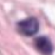
\includegraphics[width=5.5cm]{fig/cell.png}};

		% Centroid placed at cell center (image is 55px, displayed as 5.5cm)
		% Centroid at pixel (28,26) -- in display coords: (2.8, 2.9)
		% With anchor south west at (-2.75,-2.75): (2.8-2.75, 2.9-2.75) = (0.05, 0.15)
		\coordinate (CC) at (0.05, 0.15);
		\fill[red] (CC) circle (1.5pt);

		% 12 rays using polar coordinates from centroid (TUNE THESE)
		% Cell diameter ~20px -- radius ~10px -- ~1.0cm in display
		% Format: (angle:distance in cm)
		\coordinate (C0)  at ($(CC) + (  0:1.05)$);
		\coordinate (C1)  at ($(CC) + ( 30:1.10)$);
		\coordinate (C2)  at ($(CC) + ( 60:1.05)$);
		\coordinate (C3)  at ($(CC) + ( 90:0.90)$);
		\coordinate (C4)  at ($(CC) + (120:0.75)$);
		\coordinate (C5)  at ($(CC) + (150:1.05)$);
		\coordinate (C6)  at ($(CC) + (180:1.05)$);
		\coordinate (C7)  at ($(CC) + (210:1.05)$);
		\coordinate (C8)  at ($(CC) + (240:0.95)$);
		\coordinate (C9)  at ($(CC) + (270:1.00)$);
		\coordinate (C10) at ($(CC) + (300:1.05)$);
		\coordinate (C11) at ($(CC) + (330:1.10)$);

		% Rays from centroid
		\foreach \i in {0,...,11} {
			\draw[->, red!60, dashed, thin] (CC) -- (C\i);
		}

		% Polygon outline on cell
		\draw[green!70!black, thick] (C0) -- (C1) -- (C2) -- (C3) -- (C4)
			-- (C5) -- (C6) -- (C7) -- (C8) -- (C9)
			-- (C10) -- (C11) -- cycle;

		% Vertex dots
		\foreach \i in {0,...,11} {
			\fill[green!70!black] (C\i) circle (1.0pt);
		}

	\end{scope}
	\end{tikzpicture}
}
\caption{Star-convex polygon defined by centroid $\mathbf{c}$ and radial ray distances $d_i$ at fixed angular intervals $\theta_i$, forming a dense boundary representation from polar coordinates.}
\label{fig:raycast}
\end{figure}

The model parameterized each nucleus as a star-convex polygon defined by a centroid $(x, y)$ and $N$ radial ray distances $\{d_1, d_2, \ldots, d_N\}$ emanating at fixed angular intervals. The angular convention used $\theta_1 = 0^{\circ}$ along the positive $x$-axis, increasing counter-clockwise with spacing $\Delta\theta = 360^{\circ} / N$. The PanNuke configuration set $N = 64$ rays. Compared with standard bounding-box output $(x, y, w, h)$, the raycast representation captured the actual cell boundary geometry with only modest additional parameters per detection.

\subsection{Network Architecture}

\begin{figure*}[htbp]
\centering
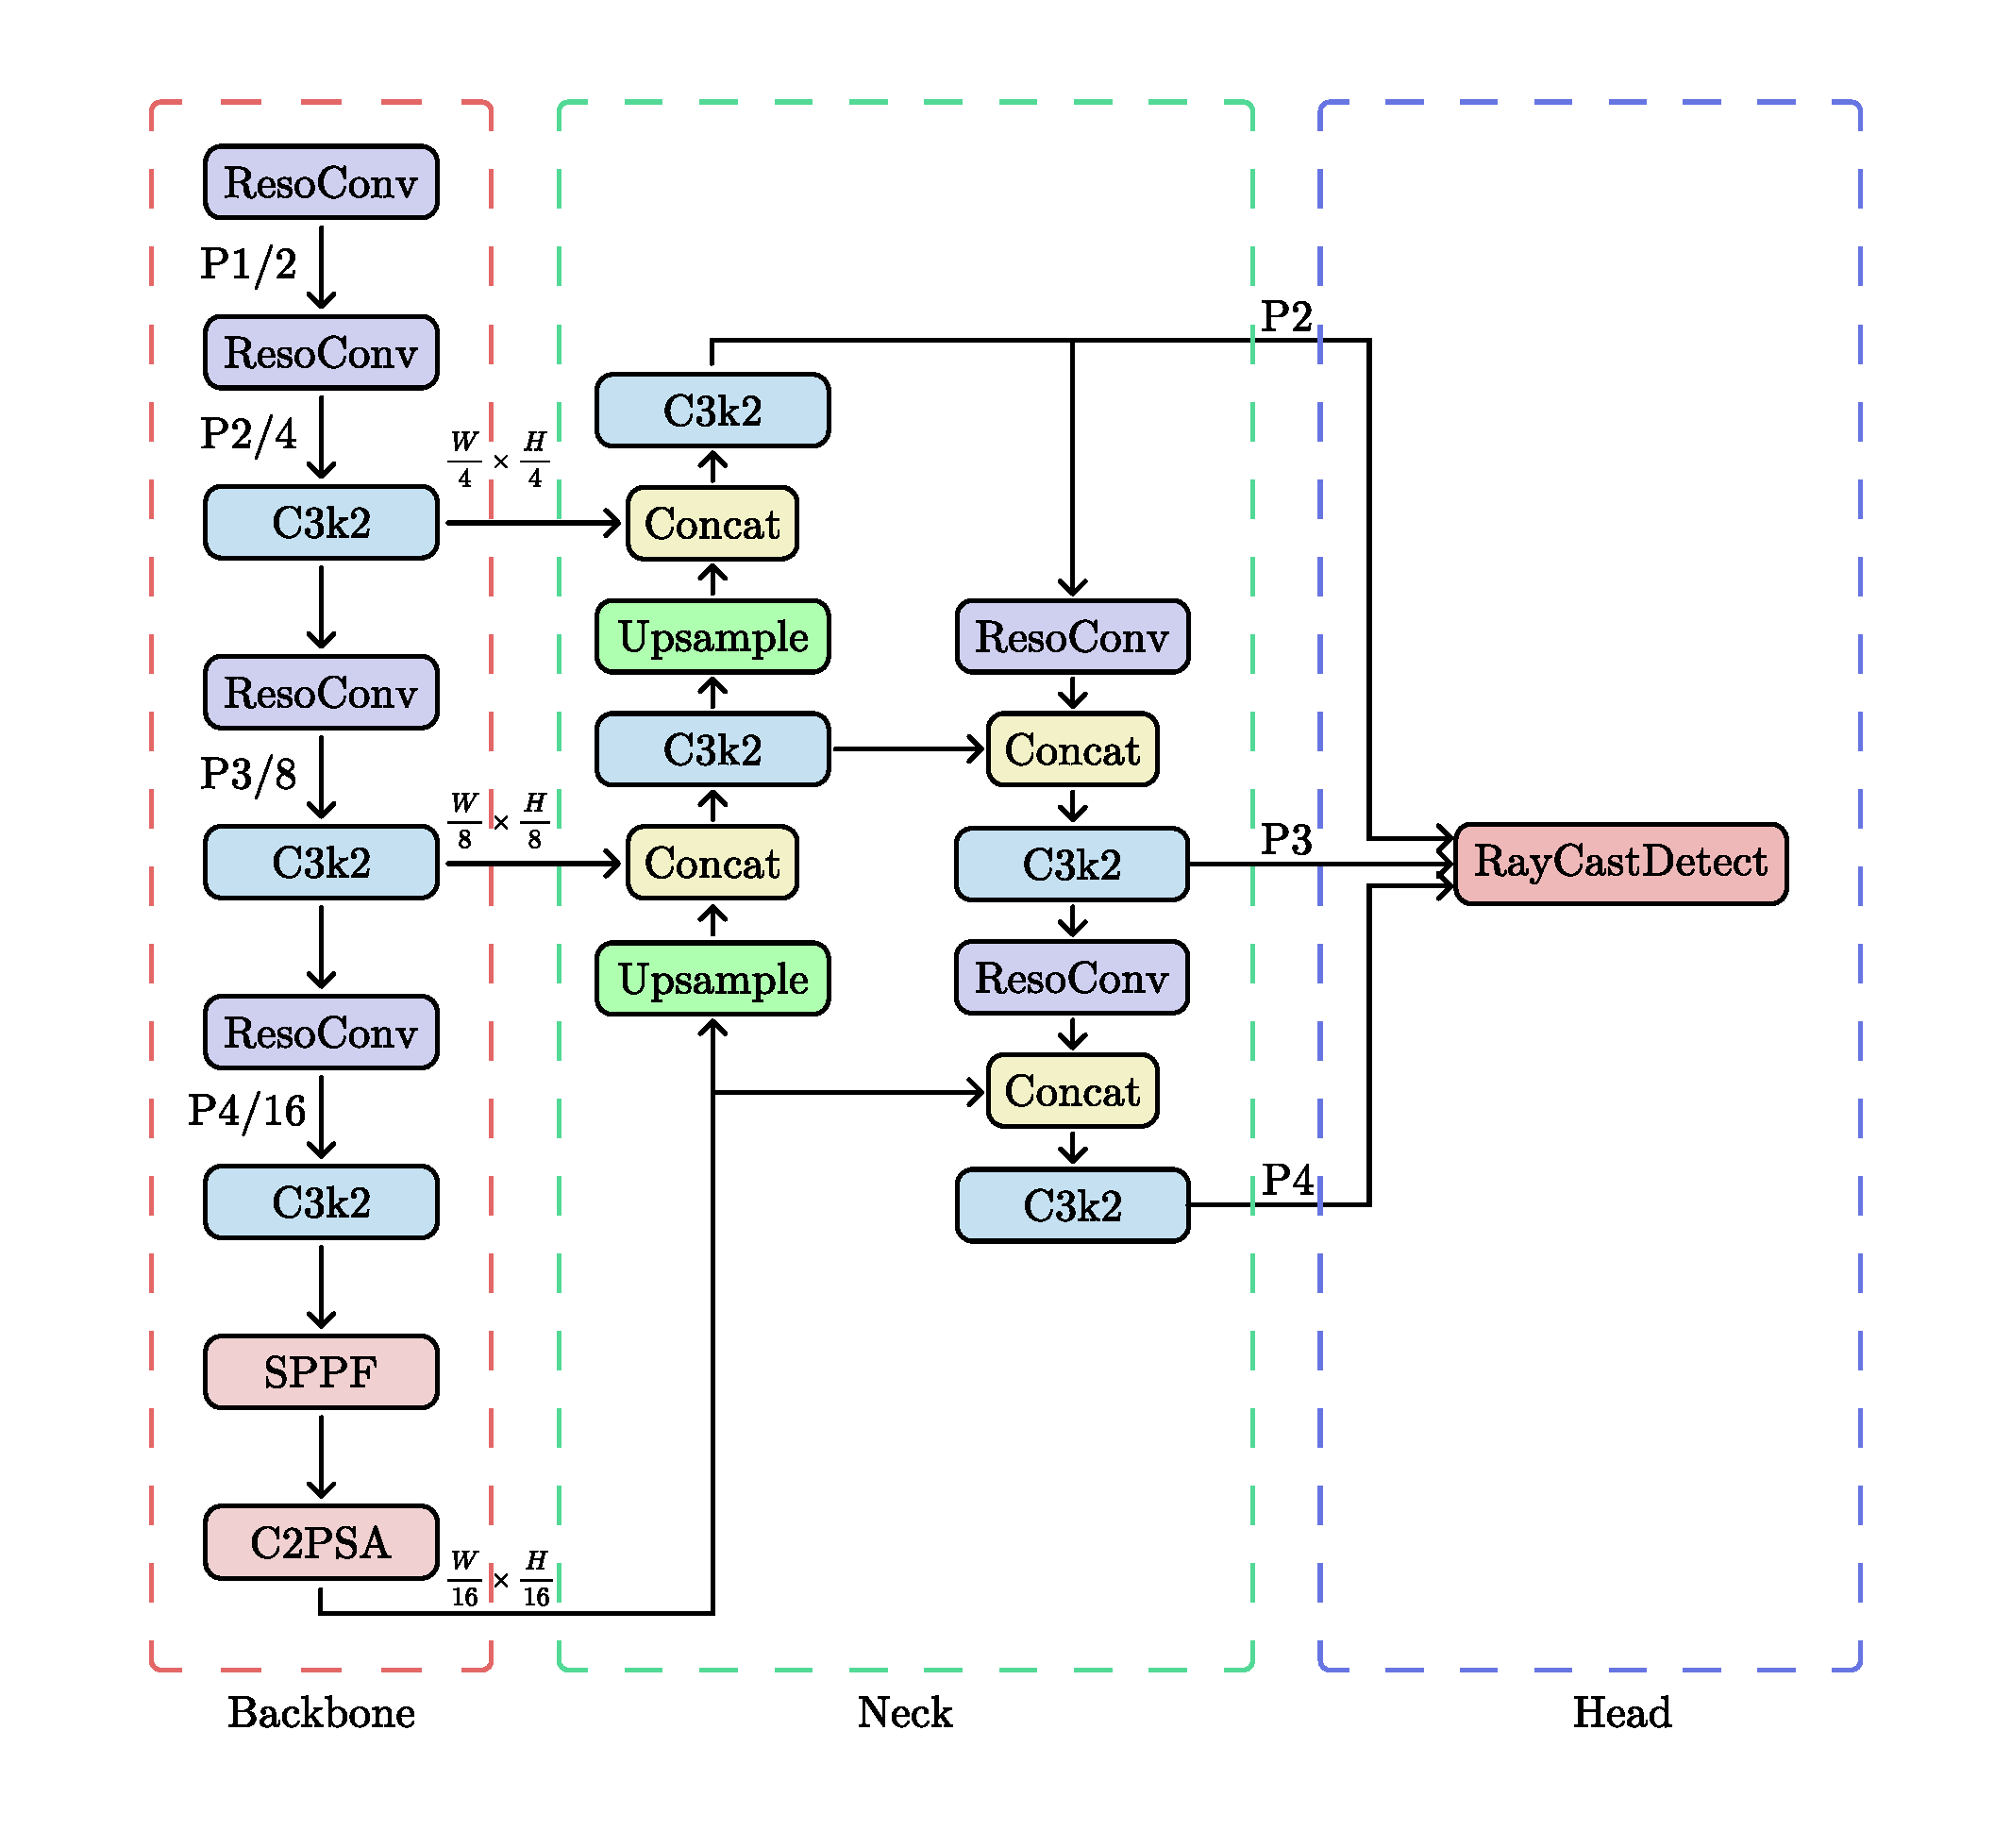
\includegraphics[width=0.6\textwidth]{fig/raycasted.pdf}
\caption{RayCastED model architecture. The backbone uses ResoConv blocks with Haar discrete wavelet transform for boundary-preserving downsampling, supporting a P2--P5 feature pyramid. The neck follows an FPN-PAN design with top-down upsampling and bottom-up aggregation. The head applies RayCastDetect with RayRefinement blocks for polygon regression at P3 (S), P4 (M), and P5 (L) scales.}
\label{fig:raycasted}
\end{figure*}

The architecture followed a backbone-neck-head design built on a YOLO26-derived fully convolutional detection framework~\cite{sapkota2025yolo26}, with all bounding-box regression components replaced by polygon prediction. Three model variants were developed: RayCastED-S (0.81M parameters), RayCastED-B (2.6M), and RayCastED-L (9.44M), scaling backbone width and depth.

\textbf{Backbone.} The backbone employed a P2-P3-P4 feature pyramid at strides 4, 8, and 16, rather than the conventional P3-P4-P5 (strides 8, 16, 32). Since histopathology tiles at $256 \times 256$ pixels typically contained $\sim$200 nuclei, the standard P3-P4-P5 pyramid provided only 1{,}344 anchors, causing multiple nuclei to collide on the same anchor. The P2-P3-P4 configuration yielded 5{,}376 anchors, reducing oversubscription from $3\times$ to $0.74\times$. Downsampling was performed by ResoConv blocks, which replaced strided convolutions with a Haar (db1) discrete wavelet transform: four subbands (LL, LH, HL, HH) were extracted via depthwise convolution with fixed Haar filters, concatenated, passed through Squeeze-and-Excitation, and projected through a $1 \times 1$ convolution. Feature extraction used C3k2 blocks, with spatial pyramid pooling (SPPF) and positional attention (C2PSA) at the deepest level.

\textbf{Neck.} An FPN-PAN (Feature Pyramid Network with Path Aggregation) operated at the P2, P3, and P4 scales. The upsampling path aggregated deep features with shallow features via nearest-neighbor upsampling, concatenation, and C3k2 fusion. The PAN downsample path used ResoConv blocks to propagate high-resolution features downward.

\textbf{Detection head.} Each scale received a dedicated polygon regression stack: two $3 \times 3$ convolutions, a RayRefinementBlock, and a $1 \times 1$ projection. The RayRefinementBlock applied $3 \times 3$ depthwise convolution with GroupNorm and SiLU activation in a residual configuration, blending spatially neighboring features before committing to ray predictions and reducing jagged boundary outputs. The head produced $2 + N$ outputs per anchor: a centroid offset $(x, y)$ decoded through sigmoid activation and $N$ ray distances decoded through softplus to enforce strict positivity. Distribution Focal Loss (DFL) regression was removed entirely, as it held no meaning for polar coordinate outputs. An auxiliary centroid head provided a lightweight $1 \times 1$ convolution bypass that delivered direct backbone-to-centroid gradients, combating attenuation through the deep head stack. The head was initialized with ray biases calibrated for approximately 15-pixel radius cells.

\subsection{Loss Functions}

The training objective combined five loss terms:
\begin{equation}
L = \lambda_{cls} L_{cls} + \lambda_{xy} L_{xy} + \lambda_{L1} L_{L1} + \lambda_{piou} L_{PIoU} + \lambda_{s} L_{smooth}
\end{equation}
with weights $\lambda_{cls} = 2.0$, $\lambda_{xy} = 500.0$, $\lambda_{L1} = 14.0$, and $\lambda_{piou} = 3.0$; $\lambda_{s}$ was annealed from 0 to 3.0 over the first 40\% of training. Each branch (O2M and O2O) computed this loss independently, combined via the O2M/O2O weight schedule.

The classification loss differed between branches. The O2M head used focal loss ($\gamma = 2.0$, $\alpha = 0.75$) with background subsampling at a 3:1 ratio of background to foreground anchors, suppressing the dominant background gradient signal. The O2O head, employing the split classification design, applied focal loss on the binary foreground/background head across all anchors and binary cross-entropy on the multiclass head restricted to foreground anchors only; the one-to-one assignment already eliminated the foreground--background imbalance.

The centroid loss $L_{xy}$ applied Huber loss ($\delta = 0.05$) on normalized grid-cell offsets. The high weight $\lambda_{xy} = 500$ compensated for gradient attenuation caused by the sigmoid activation, stride multiplication, and pixel-space normalization that the offsets undergo during decoding.

The ray distance loss $L_{L1}$ was the most distinctive component. During inference, ground-truth ray distances were computed by casting rays from the annotation centroid to the polygon boundary. During training, this same raycasting operation was reformulated as a differentiable Cramer's rule solver that computed analytical ray distances from the \emph{predicted} centroid (with gradients detached) to the ground-truth polygon boundary. The loss was evaluated in log-space:
\begin{equation}
L_{L1} = \frac{1}{R} \sum_{i=1}^{R} |\log(\hat{d}_i + \varepsilon) - \log(d_i^{\text{analytical}} + \varepsilon)|
\end{equation}
This analytical recomputation coupled centroid accuracy with ray supervision: the ray head was judged against geometrically correct targets for the position where the model placed the centroid, rather than against static targets from the ground-truth centroid, preventing conflicting gradient signals. Log-space evaluation provided scale-invariant gradients across small and large nuclei.

The PolarIoU loss provided shape-aware geometric supervision. Following PolarMask~\cite{xie2019polarmask}, each nucleus was decomposed into $R$ triangular sectors with area $S_i = \tfrac{1}{2} \sin(2\pi/R) \cdot d_i d_{i+1}$. The sector-area formulation coupled adjacent rays through the product $d_i d_{i+1}$, unlike the original per-ray PolarMask formulation that treated each distance independently. The PolarIoU was:
\begin{equation}
IoU_{polar} = \frac{\sum_{i=0}^{R-1} \min(d_i, \hat{d}_i) \cdot \min(d_{i+1}, \hat{d}_{i+1})}{\sum_{i=0}^{R-1} \max(d_i, \hat{d}_i) \cdot \max(d_{i+1}, \hat{d}_{i+1})}
\end{equation}
with $L_{PIoU} = -\log(IoU_{polar})$. The PolarIoU was computed using analytical ground-truth rays derived from the predicted centroid (consistent with $L_{L1}$), rather than static ground-truth rays as in PolarMask.

The smoothness loss applied a 1D discrete Laplacian $[-1, 2, -1]$ on the circular sequence of ray distances with cyclic indexing:
\begin{equation}
L_{smooth} = \frac{1}{R} \sum_{i=0}^{R-1} |d_{i+1} - 2d_i + d_{i-1}|
\end{equation}
The L1 norm was chosen over L2 for sparsity: along sections where the boundary evolved linearly, the Laplacian vanished exactly, while sharp corners at specific orientations incurred a bounded penalty. This loss penalized zigzag artifacts without pushing predictions toward any particular shape. The weight $\lambda_{s}$ was annealed from 0 to 3.0 over the first 40\% of training, allowing the model to learn coarse shape before refining boundary regularity.

\subsection{End-to-End Assignment}

To eliminate NMS dependency, the model employed a dual-assignment training strategy with two parallel instances of RayCastAssigner, which extended task-aligned matching by replacing standard IoU with PolarIoU in the alignment metric. The one-to-many (O2M) branch used $\text{topk}=15$ and $\text{topk}_2=15$ for dense multi-anchor supervision, while the one-to-one (O2O) branch used $\text{topk}=7$ and $\text{topk}_2=3\rightarrow 1$ (annealed over training) to select the single best anchor per ground truth for NMS-free inference.

Both branches shared the same alignment metric form:
\begin{equation}
t = s^{\alpha} \cdot \text{PolarIoU}^{\beta} \cdot \exp\!\left(\frac{-d^2}{2\sigma^2}\right)
\end{equation}
where $s$ denoted the classification score, $\alpha=0.5$, $d$ the centroid-to-anchor distance, and $\sigma$ the per-nucleus radius computed as the 75th-percentile non-zero ray distance. The O2M branch used $\beta=2.0$, rewarding well-shaped polygon predictions during early training. The O2O branch used $\beta=0$, reducing the metric to pure classification-only matching ($s^{\alpha} \cdot \exp(-d^2/2\sigma^2)$). This matched inference conditions, where no localization feedback is available to resolve assignment ambiguity, creating a self-reinforcing dynamic in which higher classification confidence yields better assignments and stronger classification gradients.

Three annealing schedules progressively shifted the training objective toward the O2O-only inference regime. The O2M and O2O branch weights transitioned linearly from $(0.8, 0.2)$ to $(0.1, 0.9)$. The O2O $\text{topk}_2$ parameter annealed from 3 to 1, allowing multiple positive anchors per ground truth during early feature learning before converging to strict bipartite matching. The smoothness loss weight $\lambda_s$ ramped from 0 to 3 over the first 40\% of training. At inference, the O2M head was discarded via fusion, leaving only the O2O head for NMS-free prediction.

\section{Results}

This section presents experimental results on PanNuke 3-fold cross-validation~\cite{gamper2020pannuke}, edge deployment latency, and ablation studies. All tables in this section report the mean across folds.

\subsection{Evaluation Setup}

Evaluation followed a 3-fold cross-validation protocol on PanNuke, with each fold serving as the test set in turn. Six baseline methods were compared: StarDist~\cite{schmidt2018cell}, CPP-Net (ResNet50)~\cite{chen2023cppnet}, CellViT-SAM-H~\cite{horst2023cellvit}, LKCell-L~\cite{cui2024lkcell}, HoVer-NeXt~\cite{baumann2024hovernext}, and LSP-DETR~\cite{pekar2026lsp}. RayCastED predictions used a confidence threshold of 0.20. All predictions were rasterized to binary masks, with the largest mask assigned to overlapping pixels.

Panoptic quality metrics (bPQ, mPQ) employed Hungarian matching at $\text{IoU} \geq 0.5$. Detection metrics (F1, precision, recall) used centroid-based matching with a 12-pixel distance threshold. Model selection was governed by the fitness function $0.7 \cdot \text{bPQ} + 0.3 \cdot \text{mAP}_{50}$. All RayCastED variants shared $O(n)$ linear complexity, with inference determined solely by the fixed anchor grid at resolutions $64 \times 64$, $32 \times 32$, and $16 \times 16$.

\subsection{Comparison with State-of-the-Art}

\begin{table}[H]
\centering
\caption{Model complexity and time complexity. $n =$ image size (pixels), $k =$ number of predicted instances.}
\label{tab:benchmark-efficiency}
\begin{tabular}{l r r l}
\hline
\textbf{Method} & \textbf{Params (M)} & \textbf{GFLOPs} & \textbf{Time Complexity} \\
\hline
StarDist~\cite{schmidt2018cell}    & 32.3  & 35   & $O(n + k^2)$ \\
CPP-Net~\cite{chen2023cppnet}      & 34.7  & 30   & $O(n + k^2)$ \\
HoVer-NeXt~\cite{baumann2024hovernext} & 36.1  & 24   & $O(n \log n + kn)$ \\
LKCell~\cite{cui2024lkcell}        & 699.7 & 214  & $O(n \log n + kn)$ \\
LSP-DETR~\cite{pekar2026lsp}       & 45.0  & 26   & $O(n)$ \\
RayCastED-S & \textbf{0.81}  & \textbf{1.38}  & $O(n)$ \\
RayCastED-B & 2.60   & 5.52  & $O(n)$ \\
RayCastED-L & 9.44   & 12.42 & $O(n)$ \\
\hline
\end{tabular}
\end{table}


Table~\ref{tab:benchmark-efficiency} summarizes parameter counts, GFLOPs, and asymptotic time complexity. RayCastED-S (0.81M parameters, 1.38 GFLOPs) was over 40$\times$ smaller than the next-lightest baseline (StarDist, 32.3M) and approximately 860$\times$ smaller than LKCell. RayCastED-L (9.44M) remained 3--5$\times$ lighter than the baseline cluster (32--45M). The entire RayCastED family shared $O(n)$ linear complexity with LSP-DETR, a consequence of the post-hoc-processing-free design. In contrast, StarDist and CPP-Net incurred $O(n + k^2)$ from per-instance NMS, while LKCell and HoVer-NeXt paid $O(n \log n + kn)$ for watershed post-processing.

\begin{table*}[t]
\centering
\caption{Per-tissue bPQ and mPQ across 19 PanNuke organ types. Best per row in bold.}
\label{tab:per-tissue}
\resizebox{\textwidth}{!}{%
\renewcommand{\arraystretch}{1.15}
\begin{tabular}{l r M r M r M r M r M r M r M r M r M}
\hline
\textbf{Tissue} & \multicolumn{2}{c}{\textbf{StarDist}} & \multicolumn{2}{c}{\textbf{CPP-Net}} & \multicolumn{2}{c}{\textbf{CellViT}} & \multicolumn{2}{c}{\textbf{LKCell}} & \multicolumn{2}{c}{\textbf{HoVer-NeXt}} & \multicolumn{2}{c}{\textbf{LSP-DETR}} & \multicolumn{2}{c}{\textbf{RC-S}} & \multicolumn{2}{c}{\textbf{RC-B}} & \multicolumn{2}{c}{\textbf{RC-L}} \\
 & bPQ & mPQ & bPQ & mPQ & bPQ & mPQ & bPQ & mPQ & bPQ & mPQ & bPQ & mPQ & bPQ & mPQ & bPQ & mPQ & bPQ & mPQ \\
\hline
Adrenal Gland & 0.636 & 0.487 & 0.689 & 0.501 & 0.679 & 0.494 & 0.698 & 0.517 & 0.624 & 0.432 & 0.656 & 0.498 & 0.583 & 0.482 & 0.594 & 0.459 & 0.620 & \textbf{0.569} \\
Bile Duct      & 0.710 & 0.461 & 0.713 & 0.475 & 0.708 & 0.485 & 0.710 & 0.490 & 0.693 & 0.462 & 0.720 & 0.494 & 0.630 & 0.463 & 0.655 & 0.486 & 0.657 & \textbf{0.506} \\
Bladder        & 0.652 & 0.491 & 0.686 & 0.514 & 0.684 & \textbf{0.523} & 0.690 & 0.512 & 0.680 & 0.508 & 0.680 & 0.507 & 0.610 & 0.464 & 0.645 & 0.503 & 0.645 & 0.512 \\
Breast         & 0.636 & 0.466 & 0.653 & 0.479 & 0.640 & 0.473 & 0.652 & 0.488 & 0.627 & 0.444 & 0.639 & 0.477 & 0.573 & 0.459 & 0.598 & 0.477 & 0.597 & \textbf{0.529} \\
Cervix         & 0.697 & 0.476 & 0.725 & 0.487 & 0.725 & 0.512 & 0.715 & \textbf{0.513} & 0.693 & 0.477 & 0.691 & 0.499 & 0.634 & 0.463 & 0.668 & 0.477 & 0.658 & 0.492 \\
Colon          & 0.689 & 0.491 & 0.714 & 0.504 & 0.703 & 0.515 & 0.711 & \textbf{0.519} & 0.687 & 0.497 & 0.705 & 0.496 & 0.614 & 0.477 & 0.657 & 0.498 & 0.656 & 0.517 \\
Esophagus      & 0.714 & 0.494 & 0.725 & 0.516 & 0.711 & 0.515 & 0.716 & \textbf{0.521} & 0.704 & 0.499 & 0.713 & 0.510 & 0.634 & 0.476 & 0.665 & 0.510 & 0.664 & 0.519 \\
Head \& Neck   & 0.641 & 0.449 & 0.644 & 0.460 & 0.645 & \textbf{0.483} & 0.651 & 0.480 & 0.621 & 0.451 & 0.640 & 0.453 & 0.565 & 0.449 & 0.587 & 0.453 & 0.593 & 0.472 \\
Kidney         & 0.649 & 0.457 & 0.672 & 0.480 & 0.672 & 0.488 & 0.666 & \textbf{0.495} & 0.640 & 0.455 & 0.665 & 0.478 & 0.592 & 0.441 & 0.610 & 0.474 & 0.615 & 0.487 \\
Liver          & 0.659 & 0.500 & 0.683 & 0.520 & 0.681 & 0.525 & 0.686 & 0.532 & 0.652 & 0.488 & 0.667 & 0.511 & 0.621 & 0.502 & 0.641 & 0.522 & 0.630 & \textbf{0.545} \\
Lung           & 0.641 & 0.434 & 0.658 & 0.450 & 0.660 & 0.458 & 0.662 & 0.456 & 0.634 & 0.431 & 0.657 & 0.449 & 0.582 & 0.417 & 0.605 & 0.440 & 0.606 & 0.448 \\
Ovarian        & 0.681 & 0.478 & 0.689 & 0.484 & 0.681 & \textbf{0.508} & 0.697 & 0.502 & 0.664 & 0.479 & 0.682 & 0.490 & 0.601 & 0.453 & 0.631 & 0.481 & 0.631 & 0.497 \\
Pancreatic     & 0.654 & 0.473 & 0.664 & 0.470 & 0.668 & 0.489 & 0.675 & 0.502 & 0.648 & 0.473 & 0.663 & \textbf{0.522} & 0.573 & 0.439 & 0.605 & 0.472 & 0.603 & 0.485 \\
Prostate       & 0.668 & 0.470 & 0.677 & 0.487 & 0.677 & 0.494 & 0.682 & \textbf{0.503} & 0.644 & 0.481 & 0.675 & 0.475 & 0.584 & 0.435 & 0.616 & 0.470 & 0.611 & 0.482 \\
Skin           & 0.662 & 0.457 & 0.662 & 0.471 & 0.670 & \textbf{0.488} & 0.670 & 0.482 & 0.631 & 0.449 & 0.669 & 0.470 & 0.593 & 0.459 & 0.609 & 0.477 & 0.615 & 0.487 \\
Stomach        & 0.697 & 0.517 & 0.707 & 0.525 & 0.699 & 0.544 & 0.705 & \textbf{0.546} & 0.681 & 0.514 & 0.696 & 0.518 & 0.608 & 0.504 & 0.646 & 0.529 & 0.644 & 0.543 \\
Testis         & 0.688 & 0.488 & 0.701 & 0.498 & 0.697 & 0.507 & 0.706 & \textbf{0.512} & 0.670 & 0.488 & 0.702 & 0.491 & 0.597 & 0.467 & 0.636 & 0.493 & 0.637 & 0.506 \\
Thyroid        & 0.689 & 0.481 & 0.705 & 0.488 & 0.701 & 0.495 & 0.696 & \textbf{0.509} & 0.673 & 0.462 & 0.692 & 0.478 & 0.610 & 0.467 & 0.636 & 0.487 & 0.636 & 0.507 \\
Uterus         & 0.652 & 0.456 & 0.663 & 0.465 & 0.663 & 0.478 & 0.677 & 0.487 & 0.635 & 0.458 & 0.656 & \textbf{0.489} & 0.565 & 0.432 & 0.600 & 0.461 & 0.609 & 0.478 \\
\hline
\textbf{AVG}    & 0.669 & 0.474 & 0.680 & 0.485 & 0.679 & 0.498 & \textbf{0.684} & \textbf{0.504} & 0.656 & 0.477 & 0.675 & 0.482 & 0.598 & 0.456 & 0.621 & 0.480 & 0.621 & 0.497 \\
\textbf{STD}    & 0.033 & 0.050 & 0.035 & 0.052 & 0.032 & 0.041 & 0.033 & 0.047 & 0.037 & \textbf{0.040} & \textbf{0.030} & 0.046 & 0.068 & 0.052 & 0.062 & 0.046 & 0.062 & 0.048 \\
\hline
\end{tabular}
}
\end{table*}

Table~\ref{tab:per-tissue} reports per-tissue bPQ and mPQ across all 19 PanNuke organ types. LKCell achieved the highest overall bPQ (0.684) and mPQ (0.504), benefiting from its 699.7M-parameter capacity. CellViT (0.679/0.498) and CPP-Net (0.680/0.485) followed closely. RayCastED-L ranked fourth on mPQ (0.497) while matching the lowest per-tissue mPQ standard deviation (0.048, tied with HoVer-NeXt at 0.040), indicating the most consistent panoptic quality across heterogeneous tissue types at its parameter tier. RayCastED-L attained the best mPQ on five organs where boundary fidelity proved decisive: Adrenal Gland (0.569), Bile Duct (0.506), Breast (0.529), Liver (0.545), and Thyroid (0.507).

\subsection{Edge Deployment}

\begin{table}[H]
\centering
\caption{Edge deployment of RayCastED-B across GPU and embedded platforms. PanNuke test set, batch size 1.}
\label{tab:edge}
\resizebox{\columnwidth}{!}{%
\begin{tabular}{l r r r r r r}
\hline
\textbf{Config} & \textbf{bPQ} & \textbf{mPQ} & \textbf{F1} & \textbf{P} & \textbf{R} & \textbf{Time (ms)} \\
\hline
RTX 5070 Ti, PyTorch  & 0.6024 & 0.4526 & 0.7409 & 0.7419 & 0.7400 & 3.59 \\
RTX 5070 Ti, TensorRT & 0.6003 & 0.4735 & 0.7745 & 0.8067 & \textbf{0.7448} & \textbf{2.70} \\
Jetson Orin Nano, ONNX & 0.5986 & 0.4763 & 0.7748 & 0.8169 & 0.7368 & 88.2 \\
Jetson Orin Nano, TF32 & \textbf{0.6118} & \textbf{0.4897} & 0.7749 & \textbf{0.8170} & 0.7369 & 38.1 \\
Jetson Orin Nano, FP16 & 0.6112 & 0.4894 & \textbf{0.7753} & 0.8140 & 0.7401 & 29.2 \\
RTX 2080 Super, TensorRT & 0.5983 & 0.4746 & 0.7746 & 0.8149 & 0.7381 & 38.8 \\
\hline
\end{tabular}
}
\end{table}


Table~\ref{tab:edge} presents RayCastED-B inference across six configurations. On the RTX 5070 Ti, PyTorch achieved near-exact predicted nuclei count (65{,}679 of 65{,}847) in 3.59 ms/image, while TensorRT reduced latency to 2.70 ms/image. On the Jetson Orin Nano, TensorRT FP16 reached 29.2 ms/image, providing viable real-time inference on an embedded platform.

An unexpected result emerged: the Jetson Orin Nano with TensorRT (both TF32 and FP16) produced consistently higher bPQ and mPQ than the RTX 5070 Ti desktop. This phenomenon was not observed on the RTX 2080 Super (bPQ~=~0.5983, mPQ~=~0.4746, matching the desktop baseline). The parity between TF32 and FP16 rules out quantization as the cause. The most plausible explanation is an architecture-specific TensorRT graph restructure that rearranges the computational graph for the Orin's Ampere-derived cores, incidentally improving numerical fidelity---an artifact not reproducible on older GPU architectures.

\subsection{Ablation Studies}

\begin{table}[htbp]
\centering
\caption{Ablation on number of rays $R$. All experiments use RayCastED-B with identical hyperparameters.}
\label{tab:ablation-rays}
\begin{tabular}{l r r r r r}
\hline
$\boldsymbol{R}$ & \textbf{bPQ} & \textbf{mPQ} & \textbf{F1} & \textbf{P} & \textbf{R} \\
\hline
8  & 0.5902 & 0.4394 & 0.7373 & 0.7334 & \textbf{0.7412} \\
16 & 0.6019 & \textbf{0.4606} & 0.7387 & 0.7393 & 0.7381 \\
32 & \textbf{0.6040} & 0.4533 & 0.7396 & \textbf{0.7455} & 0.7339 \\
64 & 0.6024 & 0.4526 & \textbf{0.7409} & 0.7419 & 0.7400 \\
\hline
STD & 0.0063 & 0.0088 & 0.0015 & 0.0051 & 0.0032 \\
\hline
\end{tabular}
\end{table}


\begin{table}[htbp]
\centering
\caption{Ablation on wavelet transform in ResoConv blocks. All experiments use RayCastED-B, $R=64$.}
\label{tab:ablation-wavelet}
\begin{tabular}{l r r r r r}
\hline
\textbf{Wavelet} & \textbf{bPQ} & \textbf{mPQ} & \textbf{F1} & \textbf{P} & \textbf{R} \\
\hline
Haar (db1)       & \textbf{0.6024} & \textbf{0.4526} & \textbf{0.7409} & \textbf{0.7419} & \textbf{0.7400} \\
Daubechies-2 (db2) & 0.6001 & 0.4435 & 0.7328 & 0.7269 & 0.7388 \\
Daubechies-4 (db4) & 0.5905 & 0.4379 & 0.7148 & 0.7046 & 0.7252 \\
\hline
\end{tabular}
\end{table}


Table~\ref{tab:ablation-rays} evaluates RayCastED-B with $R \in \{8, 16, 32, 64\}$ rays. The overall standard deviation across ray counts was small (bPQ STD~=~0.0063, F1 STD~=~0.0015), indicating modest influence on downstream metrics. Notably, mPQ was non-monotonic with respect to $R$, peaking at $R = 16$ (0.4606) rather than at $R = 64$. This pattern suggests that the small 2.6M-parameter backbone converges to an approximately elliptical prior regardless of ray density, consistent with the well-established observation that nuclear membranes are mechanically constrained to near-convex shapes by the nuclear lamina. The $R = 64$ default was retained to maximize boundary fidelity for future larger backbones.

Table~\ref{tab:ablation-wavelet} compares three wavelet transforms within ResoConv blocks. The Haar wavelet (db1) swept all five metrics (bPQ~=~0.6024, mPQ~=~0.4526, F1~=~0.7409, P~=~0.7419, R~=~0.7400), outperforming Daubechies-2 (db2) and Daubechies-4 (db4) by increasing margins. The degradation from db1 to db4 (bPQ drop of 0.0119, F1 drop of 0.0261) confirms that longer wavelet filter taps introduce excessive smoothing that attenuates fine-grained edge transitions, chromatin texture, and boundary information---precisely the high-frequency content on which the contour-based detection head depends. The Haar wavelet emerged as the single most impactful architectural choice in the entire model.

\section{Conclusion}

RayCastED demonstrates that a lightweight, fully convolutional, post-hoc-processing-free architecture can deliver competitive panoptic nuclei segmentation while enabling edge deployment. The largest variant, RayCastED-L (9.44M parameters), achieved a mean panoptic quality of 0.497 (4th overall on PanNuke 3-fold cross-validation) with the lowest per-tissue mPQ standard deviation (0.048) among models of comparable or larger size, at 3--5$\times$ fewer parameters than StarDist, CPP-Net, HoVer-NeXt, and LSP-DETR, and approximately 75$\times$ fewer than LKCell. The entire variant family shares $O(n)$ linear complexity---a direct consequence of eliminating post-hoc NMS and watershed---marking a departure from the $O(n + k^2)$ or $O(n \log n + kn)$ complexity of prior contour-based and mask-based methods.

Edge deployment confirmed that RayCastED-B achieves real-time inference on the RTX 5070 Ti (2.70 ms/image, TensorRT) and near-real-time on the Jetson Orin Nano (29.2 ms/image, FP16), establishing the feasibility of deploying contour-based nuclei detection in resource-constrained clinical settings without cloud offloading. The persistent TensorRT fidelity anomaly on Jetson Orin Nano (consistently higher bPQ/mPQ than desktop) warrants further investigation as a potential avenue for architecture-aware graph optimization.

Ablation studies identified the Haar discrete wavelet transform in ResoConv blocks as the most impactful architectural component (sweeping all five evaluation metrics over db2 and db4), while ray-count experiments revealed that current backbone capacity limits the model to an elliptical shape prior---an important insight for scaling to larger backbones with denser ray configurations. Zero-shot generalization was strong on PUMA melanoma tiles but weak on panopTILs and MoNuSAC, confirming that tissue-level and staining-protocol domain gaps require fine-tuning, even though the raycast representation itself is dataset-agnostic.


\section*{Acknowledgment}

\bibliography{references}{}
\bibliographystyle{IEEEtran}

\end{document}
